\chapter{Experimental Evaluation}
\label{cha:results}

In this chapter, all the finding will be presented during the testing phase.
% Three games were tested: the Hearts Game, the Maze Game, and the Puzzle Game. During these testings data was gathered from gameplay sessions and post-interviews with children between the age of six and seven years old.

These games were designed to help children with specific learning disabilities like dyslexia, dyscalculia, and other challenges. The tests were only made with children that were not diagnosed with LDs.

The aim is to understand how well these games engaged the children, supported their learning, and addressed their difficulties.


\newpage

\section{Testing process and limitations}

For these studies, tests were conductucted regarding three out of the five minigames developed in this project.
With the help of the teachers, Salomé Alves and Ana Cardoso, from the school EB1/JI da Portela. This school has multiple students from the first to fourth grade, having children between the ages of six to ten.
The testing scenario was done in the Class 1A, correspondant to the first graders.
The teacher played an essential role in coordinating the testing sessions, ensuring the children understood the instructions, and providing support throughout the process.

Originally, the goal of these tests were to test specifically with children who have LDs. Unfortunately, this was not possible. Due to several factors, the orienting team of the project was not able to reach a large enough group of children with LDs. Some of the challenges include the limited access to specialized schools and restrictions to obtaining parental consent for participation. We decided to carry out a test scenario with a broader group of children.

Despite the children in the current study not necessarily having LDs, it still provides us with valuable insights on the developed project. Like mentioned before, all the games share similar design, interactions, narratives and levels. The feedback received from the children, helped identify universal issues also affect children with LDs, such as the need for clearer instructions, and the effectiveness of visual aspects of the game. This feedback are directly applicable to refining all five games.

Two tests were conducted in both July and October of 2024. As the games were not all ready in July, the first round of tests only included the Hearts Game, the Maze Game, and the Puzzle Game. Only the second round included the other two games (Sounds Game and Words Game). As there were two rounds of tests, we were able to fix or add functionalities from the first one to be tested again in the other tests.

Moreover, many of the challenges observed, like motor coordination problems and the difficulty some children had in focusing, are issues that are also commonly faced by children with LDs. With this in mind, the problems identified and the corresponding improvements suggested are relevant to the target group in mind in the beginning.

\newpage
\section{Results}

In this section, it is intended to go in depth in the tests performed in the classroom. It's important to notice that, for each game, data was gathered in two batches. The first one was the observing of the children during the \textbf{gameplays} and even small conversation while the children is playing the game. The second and last part was a small post interview to gather \textbf{feedback} from the children such as pros, cons and some observations the children might have.

The informations retrieved were the following.

\paragraph{Gameplay}
\begin{itemize}
    \item Difficulties
    \item Game Score
    \item Quality
    \item Is the game easy?
    \item Comments
    \item Socializing
    \item Observations
\end{itemize}

\paragraph{Feedback}
\begin{itemize}
    \item Did you like the game?
    \item Are levels hard?
    \item Did you like all the levels?
    \item Did you like the stories?
    \item Was it hard to understand what to do?
    \item Did you learn anything?
    \item Could it be more fun? How?
    \item Would you like to play it everyday?
    \item Do you want to play it with friends?
\end{itemize}


\subsection{Maze Game Results}
The game had players move Mr. Pig through a maze, collecting items before finding the exit. As players moved to higher levels, the mazes got bigger and more complicated.

Many kids found the controls difficult. Some had trouble using the mouse, especially on larger levels. Others breezed through the early stages but struggled with the harder ones later on. This shows that while some levels were too easy for certain kids, others were quite challenging. Comments like “move, pig” and “the little pig doesn’t want to go” were common, highlighting how character movement was tricky for some. It suggests that using the mouse was a major obstacle for many of them.

Despite some difficulties, most children said they enjoyed the game. Many of them were enthusiastic, with responses like “yes, I'd play everyday”, being common. However, there were also some suggestions for improvement, such as making Mr. Pig move faster or simplifying the controls.

Overall, the Maze Game was engaging for the kids, though it highlighted issues with motor coordination, especially for those using a mouse. This shows how important it is to simplify controls for children who have motor skill challenges. The narrative—about Mr. Pig cleaning up the garbage—seemed to resonate well with the children, which kept them motivated despite the control issues.

With these issues in mind. The game's control, that was previously done just with mouse drag and dropping, was changed allowing for the users to play with the 'WASD' or arrow keys. This was done so that, if movement with the mouse is tricky the user can use other options.

During the second round of tests we noticed that the children maintained similar interest levels, with children excited to play. Nevertheless, some players found the game either too easy or too challenging. This might suggest the designing of some new levels with other difficulties. Based on observations, there was a better understanding of the games mechanics but there were still some children who had difficulties understanding them. This is something to think of when refining the game.

% Maze
    % Nao foi explicito a utilizacao de setas inves drag n drop
    % Interest and Engagement: The second round maintained similar interest levels, with children excited to play. However, some found the game either too easy or too challenging based on individual preferences and familiarity.
    % Improvements Observed: Children seemed more aware of what was expected in terms of gameplay. However, navigating the game’s interface, especially at level selection, remained a challenge.
    % Suggested Enhancements: Based on comments, simplifying controls and providing clearer guidance at the start could improve overall user experience and allow children to feel more independent.

\newpage
\subsection{Puzzle Game Results}

The Puzzle Game featured ecology-themed puzzles with three levels of difficulty to choose from. The players had to place pieces into a puzzle using a tray.

The children’s performance varied widely. Some completed the puzzles quickly, while others needed some assistance. There were also some that showed a lot of enthusiasm, mentioning that he was ''“very good at puzzles''. However, some children, didn’t notice the reference images provided, which might have made solving the puzzles easier for them.

The Puzzle Game seemed to be well received, but it was clear that some children needed more help noticing important visual cues, like the reference image. For this, the reference image was made more obvious with the help of a frame around it, making it clearerer to the users and improving the experience. The figure \ref{fig:puzzleRefImage} details the new reference image.

\begin{figure}[!h]
    \centering
    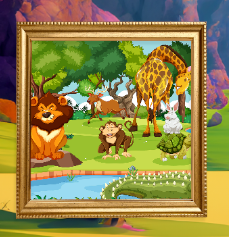
\includegraphics[width=0.3\linewidth]{Chapters/game_changes/puzzle-game-frame.png}
    \caption{Reference Image Frame}
    \label{fig:puzzleRefImage}
\end{figure}

In the second round of tests the popularity of the game was reinforced, with positive remarks on its design. After the inserting of the new reference image frame (fig. \ref{fig:puzzleRefImage}) the spotting for it was a lot clearer and easier for children too understand how it works. Besides the positive feedback there are still ways that can be adopted for a better user experience, such as a different background image that contrasts more with the game elements.
Familiarity helped children perform better, though some still felt a little lost with the controls. This issue might be present in more of the games and its solution might be applicable for all games.

Overall, the positive comments and the children’s eagerness to play again show that puzzles can be an effective way to develop problem-solving skills.

% Puzzle
    % Foi mencionado q utilizavam as setas instintivamente
% Interest and Engagement: The second round reinforced the popularity of the game, with positive remarks on its design. Children showed continued enthusiasm and enjoyment, particularly for completing the puzzles.
% Progress in Interaction and Control: Familiarity helped children perform better, though some still encountered issues with the dragging mechanism.
% Suggested Enhancements: Adding prompts or instructions on how to interact with puzzle pieces (e.g., dragging) could further reduce frustration and improve ease of use.

\newpage
\subsection{Hearts Game Results}

The Hearts Game was about collecting items and following a story as the levels got harder.

Some children had trouble concentrating and needed help, especially on the difficult levels. One child needed assistance on the third level, which she found tough. A few kids struggled with controlling the game, particularly when using the mouse.

Feedback was mixed. Two enjoyed the game and said they’d like to play it again. Others found it too hard and weren’t eager to replay. One mentioned it could be more enjoyable but didn’t offer specific suggestions. The story didn’t engage everyone; responses varied when asked, “Did you like the stories?”.

The game highlighted challenges with control and understanding. The difficulty of some levels and unclear instructions made it less fun for some children. Simplifying the controls and offering more guidance on harder levels could make the game better. However, the positive feedback from others suggests the story aspect could work well with some improvements.

After the second round of tests we could observe some children like the game but complained about its duration. After reviewing this aspect, we could see that the duration of each level is too short and should be revised. During this round we could also see some difficulties when trying to exit the game before the level was started. This can be a user experience issue and should be addressed. During the first round of tests, some children were upset of how long the story of the game is. This no longer seemed to be a problem, as the stories can be read out loud in the new version.


% Hearts
    % 1st try a historia e muito longa
    % A duracao do jogo e muito pequena
    % Houve criancas que nao conseguiam sair do jogo antes de o comecarem (Adicionar botar de voltar atras)
    % Uma crianca nao sabe o que fazer (Pedro)

% Interest and Engagement: Feedback continued to be mixed, with some children enjoying the game while others found it difficult or unappealing.
% Improvements in Comprehension and Control: Some children better understood the objectives after repeated play, though unclear instructions still posed a challenge.
% Suggested Enhancements: Simplifying story elements and providing clearer, step-by-step objectives could improve focus and understanding, especially for younger players.

\newpage
\subsection{Words Game Results}
The Words Game was designed to test the children's language and letter recognition abilities. The gameplay involved children completing words on the screen related to either ``nature objects'' or ``industrial objects'', with each category offering a distinct set of vocabulary. This game aimed to assess their familiarity with words, understanding of word construction, and ability to recognize and place letters accurately.

Children engaged actively with the Words Game, often discussing words with each other and asking peers for help if they found a word difficult. The game fostered collaboration as they compared strategies or took turns attempting words from each category.

Most children found the Words Game to be accessible and enjoyable, particularly those who enjoyed spelling and word games. They appreciated the word categories, which were relatable and easy to understand.

A few children encountered issues with specific words that contain accents in them, such as ``Árvore'' (tree). These challenges sometimes led to frustration, especially if they felt they had to start over. Despite this being good, because the game aims to improve the vocabulary and grammar, this led us to believe that maybe the order of the words in the levels might not be ordered (from easy to hard words).

The Words Game successfully engaged children in spelling and word recognition tasks, having a positive feedback. Improving the order of the levels from easy to harder, having in consideration factors like, accents and length of the word, could really increase the quality of the experience, allowing children to focus more on word completion rather than technicalities of interface interaction.


% Words
    % Foi bem recebido, causou entisiasmo e foi challenging
    % Algumas palavras estavam commo nivel baixo e tinham assentos 

% Testing Process:

% Instructions and Interaction: Before starting, children were briefed on the objective: to complete the word by selecting the correct letters. They received additional guidance on specific interactions, such as where to click or how to place letters in sequence. For children unfamiliar with accented letters, some needed clarification on how to interact with such characters.
% Socialization and Engagement: 
% Findings and Challenges:

% Feedback and Recommendations: Feedback highlighted a desire for smoother letter placement and clearer instructions regarding accents and special characters. Enhancing the precision of letter placement and incorporating subtle instructions for handling accents could improve the gameplay experience.
% 




\newpage
\subsection{Sounds Game results}

The Sounds Game was designed to test children's ability to identify and match various sounds to their corresponding instruments. The game was introduced to children in a familiar setup, where they interacted with a digital interface, listening to sounds and selecting the correct instrument on the screen. The goal was to assess not only their auditory processing skills but also how well they could differentiate sounds in a potentially distracting environment.

During gameplay, children showed high levels of interest, often engaging in friendly competition to see who could match the sound fastest. Time results were recorded to add an element of competition, which helped sustain engagement. Many children interacted with each other throughout the game, comparing their results and discussing the different sounds they encountered.

The children expressed enjoyment with the game, especially with the novelty of identifying musical instruments. This game had one of the highest engagement levels among the group.

Some children struggled when overlapping sounds or background music confused the main sounds. This issue was more pronounced for children with lesser auditory processing skills, who found it difficult to separate and identify individual sounds within a layered auditory environment.

Feedback was largely positive, but simplifying the sound environment could enhance gameplay. Recommendations included isolating sounds further and ensuring each sound was clearly distinguishable from any background noise. This could make the game even more accessible, particularly for children who may find multiple sounds distracting.
Overall, the Sounds Game demonstrated strong engagement and interest, with children responding positively to the interactive, audio-based approach. Addressing the challenge of background noise could further optimize the experience, making it accessible to a wider range of auditory processing abilities.


\newpage
\subsection{Discussion}

With the results in mind we can see both success and improvement areas. The children displayed a lot of enthusiasm, some wanting to play them regularly. The tests provided us with real feedback such as recurring issues with the control in the Maze Game for instance, that was quickly fixed after, simplifying the control schemes. Also the issue with the visual cues provided in the Puzzle Game not being well accessible by some players that was also fixed later on.


The feedback highlighted the importance of engaging content that matches the children’s interests, such as ecology and familiar characters. The games did well in capturing their attention and gave the valuable insights into how different game mechanics impact engagement and learning for kids with learning disabilities.

One common thing that happened sometimes was that the children sometimes skipped the games stories and instructions and sometimes had to come back and read it in order to know how to play the games. To simplify this, the reading out loud feature was created and set to read each game's story before starting it, along with a new button that allows for the enabling/disabiling the reading out loud (fig. \ref{fig:readInstructionsButton}).

\begin{figure}[!h]
    \centering
    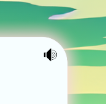
\includegraphics[width=0.1\linewidth]{Chapters/game_changes/read-sound-icon.png}
    \caption{Read Instructions Button}
    \label{fig:readInstructionsButton}
\end{figure}

% Usability Challenges: Complex controls, unclear instructions, and interface difficulties were common issues. Adding prompts and simplifying mechanics could enhance the user experience.

There were also some usability challenges regarding unclear instructions, and interface difficulties in multiple games. To later fix this each game should have in its homescreen an ``Instructions'' labeled button that provides a clear understanding of the game mechanics. Another user experience issue, that was found during the Hearts Game testing but can be applicable to any other game was the inability of exiting the game before starting any level. Some children tried clicking the ``Pause Game'' button and were met with no reaction because the level hadn't actually started. A new input should be added to the games so that exiting could be accessible from any screen. Adding this could enhance the user experience.

The second round of tests was really helpful to gather some more information on the games that were previously tested, as well as some new info on the ones that hadn't yet been exposed to players. With this new round, we found the children really excited, as they were already familiarized with the games. We could also see an improvement on some issues encountered before. Because of this, we gathered more feedback and some features and bugs to tackle in order to better increase the quality.

Overall, the enthusiasm shown by many of the children indicates that educational games have great potential to support learning when they are designed with their needs in mind.

% Interest Levels: Across all games, children showed a general enthusiasm for gameplay. They especially enjoyed aspects involving feedback, competition, and visuals.
% Socialization: The games naturally encouraged social interaction, with children engaging in supportive discussions and showing excitement for their progress.
% Potential Improvements: Simplifying controls, providing clearer guidance, and adding personalized levels could make games more accessible and enjoyable for children with different abilities and preferences.

% Maze
    % Nao foi explicito a utilizacao de setas inves drag n drop
% Puzzle
    % Foi mencionado q utilizavam as setas instintivamente
% Hearts
    % 1st try a historia e muito longa
    % A duracao do jogo e muito pequena
    % Houve criancas que nao conseguiam sair do jogo antes de o comecarem (Adicionar botar de voltar atras)
    % Uma crianca nao sabe o que fazer (Pedro)
% Sounds
    % Foi bem recebido
% Words
    % Foi bem recebido, causou entisiasmo e foi challenging
    % Algumas palavras estavam commo nivel baixo e tinham assentos 

% Discussion
    % Foi notavel q no jogos do labirinto e do puzzle nao esta explicito como jogar o jogo
    % Por isso devemos criar um novo


% Going forward, some things that would totally increase the quality of the games, would be the access for multiple languages. Right now, the games are tailored to a specific group of children and, the ability to add new levels is quite simple being a developer. This is due to the simplicity of the design of the software. Despite this, because these games are to be used in schools and medical centres, the end game is to let the teachers or doctors or anyone assisting the gameplay to children to be able to edit and create a completely different narrative for each children. What can be proposed is a new area to the main menu, where the tutor can manage each game and customize the gameplay. This could include changing the story, icons, and adding or removing levels.